
\section{Introduction}

\begin{frame}
	\frametitle{Lead Compensator vs Lag Compensator}
	\begin{block}{Closed-loop diagram}
		\begin{figure}
			\centering
			\includegraphics[width=1\linewidth]{Closed-Loop}
		\end{figure}
	\end{block}
	\begin{block}{Transfer functions}
		Lead compensator : 
		$C(s) = K\frac{s + \frac{1}{\tau}}{s + \frac{1}{\alpha\tau}}$ with $0 \textless  \alpha  \textless  1$ \\
		Lag compensator : 
		$C(s) = K\frac{s + \frac{1}{\tau}}{s + \frac{1}{\beta\tau}}$ with $\beta  \textgreater  1$ 
	\end{block}
\end{frame}

\begin{frame}
\frametitle{Lead Compensator vs Lag Compensator: zeros and poles}
\begin{block}{Transfer functions}
	Lead compensator : 
	$C(s) = K\frac{s + \frac{1}{\tau}}{s + \frac{1}{\alpha\tau}}$ with $0 \textless  \alpha  \textless  1$ \\
	Lag compensator : 
	$C(s) = K\frac{s + \frac{1}{\tau}}{s + \frac{1}{\beta\tau}}$ with $\beta  \textgreater  1$
\end{block}
\begin{block}{Zeros and poles}
	Zeros: $s = -\frac{1}{\tau}$ \\
	\vspace{0.1cm}
	Poles: $s = -\frac{1}{\alpha\tau}$ (for lead) or $s = -\frac{1}{\beta\tau}$ (for lag) \\
	\vspace{0.1cm}
	For lead compensators the pole lies more to the left in the complex plane than the zero and vice versa for lag compensators.
\end{block}
\end{frame}

\begin{frame}
\begin{block}{Important!}
There are two ways of designing this kind of compensators:
\begin{itemize}
\item making use of frequency domain tools
\item making use of root locus
\end{itemize}
In this chapter, we will only focus on {\bf frequency domain tools}.
\end{block}
\end{frame}

\section{Lead compensators}

\begin{frame}
\frametitle{Lead compensators}
	\begin{block}{Transfer function}
		$C(s) = K\frac{s + \frac{1}{\tau}}{s + \frac{1}{\alpha\tau}} =    K\alpha\frac{\tau s + 1}{\alpha\tau s + 1}$ with $0 \textless  \alpha  \textless  1$
	\end{block}
	\begin{block}{Bode Diagram}
		Example with K = 10, $\alpha$ = 0.1 and $\tau$ = 0.1 (see next slide) \\
		Magnitude of the lead compensator:
		\begin{itemize}
			\item becomes unity (= 0 dB) for small frequencies
			\item becomes 10 (= 20 dB) for high frequencies
		\end{itemize}
		$\Rightarrow$ A lead compensator is a {\bf high-pass filter}.
	\end{block}
\end{frame}

\begin{frame}
\frametitle{Lead compensators}
\begin{block}{Bode Diagram}
\begin{figure}
	\centering
	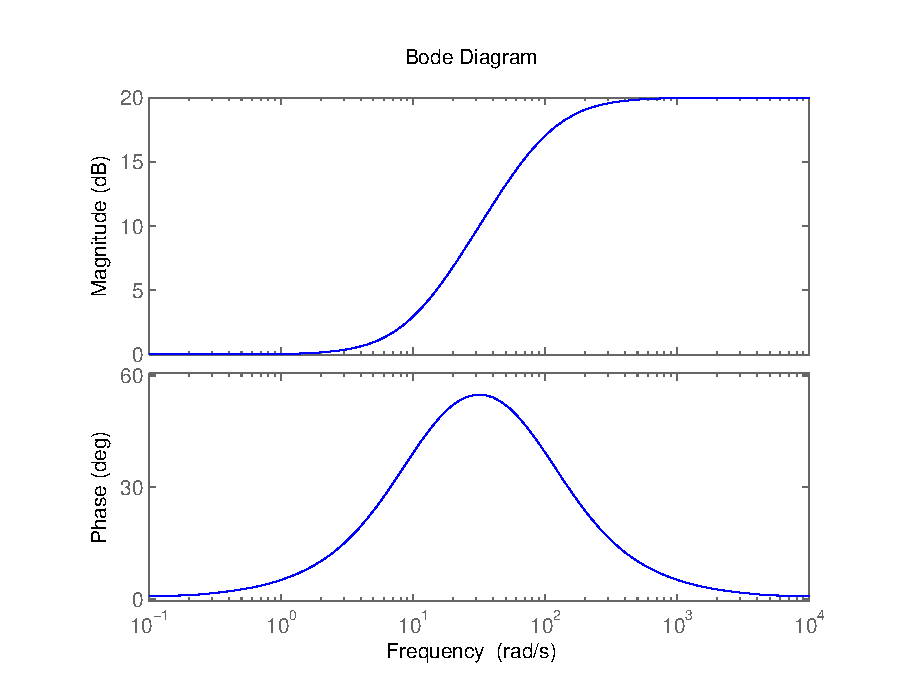
\includegraphics[width=0.7
	\linewidth]{bodeleadfilter2}
\end{figure}
\end{block}
\end{frame}

\begin{frame}
\frametitle{Lead compensators}
\begin{block}{Impact}
	\begin{itemize}
	\item Push the poles of the closed loop system to the left.
	\begin{itemize}
	\item Stabilization of the system (see root locus).
	\item Increase response speed and bandwidth.
	\end{itemize}
	\item Increase of the phase margin: the phase of the lead compensator is positive for every frequency, hence the phase will only increase.
	\end{itemize}
\end{block}
\end{frame}

\begin{frame}
	\frametitle{Design with Bode plots}
	\begin{block}{Step 1}
		\begin{itemize}
			\item Translate the steady state requirement in terms of the pertinent error constant:
			\begin{itemize}
				\item $K_p = \lim_{s \to 0} P(s)C(s)$ (position)
				\item $K_v = \lim_{s \to 0} sP(s)C(s)$ (velocity)
				\item $K_a = \lim_{s \to 0} s^2P(s)C(s)$ (acceleration)
			\end{itemize}
			\item With this $K_p/K_v/K_a$, determine $K\alpha$.
			\item Verify whether a proportional controller with gain $K\alpha$ satisfies the phase margin requirements.
		\end{itemize}
	\end{block}
\end{frame}

\begin{frame}
	\frametitle{Design with Bode plots}
	\begin{block}{Step 2}
		Determine $\phi$ as the extra phase margin (PM) we have to add to  $K\alpha P(s)$. If the PM is ok, there is not need of a lead compensator since a proportional controller with gain $K\alpha$ suffices.
	\end{block}
	\begin{block}{Step 3}
		Add $5\,^{\circ}$ to $\phi$: $\phi_m = \phi + 5\,^{\circ}$ (if $\phi_m > 60\,^{\circ}$, you will need more than one lead compensator). The addition of a lead compensator shifts the gain crossover frequency to the right and decreases the
		phase margin.
	\end{block}
\end{frame}

\begin{frame}	
	\frametitle{Design with Bode plots}
	\begin{block}{Step 4}
		Determine $\alpha$ making use of the polar plot of 
		$\frac{\alpha(j\omega\tau + 1)}{j\omega\alpha\tau + 1}$	
		\begin{figure}
			\centering
			\includegraphics[width=0.4
			\linewidth]{leadcompalphabepalen}
		\end{figure}
		$\sin\phi_m = \frac{\frac{1}{2}\left( 1 - \alpha \right)}{\frac{1}{2}\left( 1 + \alpha \right)} = \frac{1 - \alpha}{1 + \alpha} \Rightarrow \alpha = \frac{1 - \sin\phi_m}{1 + \sin\phi_m}$. Usually, $\alpha \geqslant 0.05$. \\
		We know $\alpha$ and we know $K\alpha$ (step 1), so we can calculate K.
	\end{block}
\end{frame}

\begin{frame}
	\frametitle{Design with Bode plots}
	\begin{block}{Step 5}
		Use the gain crossover frequency of P(s)C(s), denoted by $\omega_m$: \\
		\vspace{0.2 cm}
		$\mid P(j\omega_m)C(j\omega_m) \mid = 1$ \\
		\vspace{0.2 cm}
		$\mid P(j\omega_m) \mid K \frac{\sqrt{\frac{1}{\alpha\tau^2} + \frac{1}{\tau^2}}}{\sqrt{\frac{1}{\alpha\tau^2} + \frac{1}{\alpha^2\tau^2}}} = \mid P(j\omega_m) \mid K \sqrt{\alpha} = 1$ \\
		\vspace{0.2 cm}
		$20\log \mid P \left( j\omega_m \right) \mid = -20\log \left( K\sqrt{\alpha} \right)$ \\
		\vspace{0.2 cm}
		$\Rightarrow GCF \left( P(s)K\sqrt{\alpha} \right) = \omega_m$ \\
		\vspace{0.2 cm}
		The value of the tangent point $\omega_m$ can be determined from the Bode plot of $K\sqrt{\alpha}P(s)$, we know $K$ and $\alpha$ from step 4.
	\end{block}
\end{frame}

\begin{frame}\frametitle{Design with Bode plots}

\begin{columns}
	\begin{column}{.49\textwidth}
		\begin{block}{Step 6}
		The tangent point $\omega_m$ is the geometric mean (frequency scale is logarithmic!) of the two corner frequencies (zeros and poles), so
		$ \log \omega_m = \frac{1}{2}(\log \frac{1}{\tau} + \log \frac{1}{\alpha\tau})$ with $\tau = \frac{1}{\omega}$
		\\ $\Rightarrow \omega_m = \frac{1}{\sqrt{\alpha}\tau} \Rightarrow \tau = \frac{1}{\sqrt{\alpha}\omega_m}$.
		\end{block} 
	\end{column}
	
	\begin{column}{.49\textwidth}
		\begin{figure}
			\centering
			\includegraphics[width=1
			\linewidth]{tangentpointpijlen}
		\end{figure}
	\end{column}
\end{columns}

\end{frame}

\begin{frame}
	\frametitle{Design with Bode plots}
	\begin{block}{Step 7}
		Verify that the system behaves as desired.
		Check the phase margin and steady state requirement to make sure they are satisfactory. If not, repeat the design process
		by modifying the pole-zero location of the compensator until a satisfactory result
		is obtained.
	\end{block}
\end{frame}

\begin{frame}
\begin{example}
	Consider the system $P(s) = \frac{4}{s(s+2)}$ with Bode Diagram below. 
	\vspace{0.1 cm}
	We want the phase margin to be at least $50\,^{\circ}$ and the static velocity error constant $K_v = \frac{20}{sec}$.  
	\begin{figure}
		\centering
		\includegraphics[width=0.5
		\linewidth]{bodeexamplelead}
	\end{figure}
\end{example}
\end{frame}

\begin{frame}
\begin{exampleblock}{Step 1}
\begin{itemize}	
\item Steady state requirement: $K_v = \frac{20}{sec}$ \\
So, $\lim_{s \to 0} sP(s)C(s) = \lim_{s \to 0} s\frac{4}{s(s+2)}K\alpha = 2K\alpha = 20$. \\
$\Rightarrow K\alpha = 10$
\item Would a proportional controller with gain $K\alpha$ suffice? We have to take a look at the Bode Diagram of $K\alpha P(s)$ (see next slide) \\
$\Rightarrow$ It does not suffice! The phase margin is obviously smaller than $50\,^{\circ}$.
\end{itemize}
\end{exampleblock}
\begin{exampleblock}{Step 2}
	\begin{itemize}
	\item Phase margin of $K\alpha P(s) = 18\,^{\circ}$.
	\item We want a phase margin of at least $50\,^{\circ}$
	$\Rightarrow \phi = 32\,^{\circ}$.
	\end{itemize}
\end{exampleblock}
\end{frame}

\begin{frame}
	\begin{figure}
		\centering
		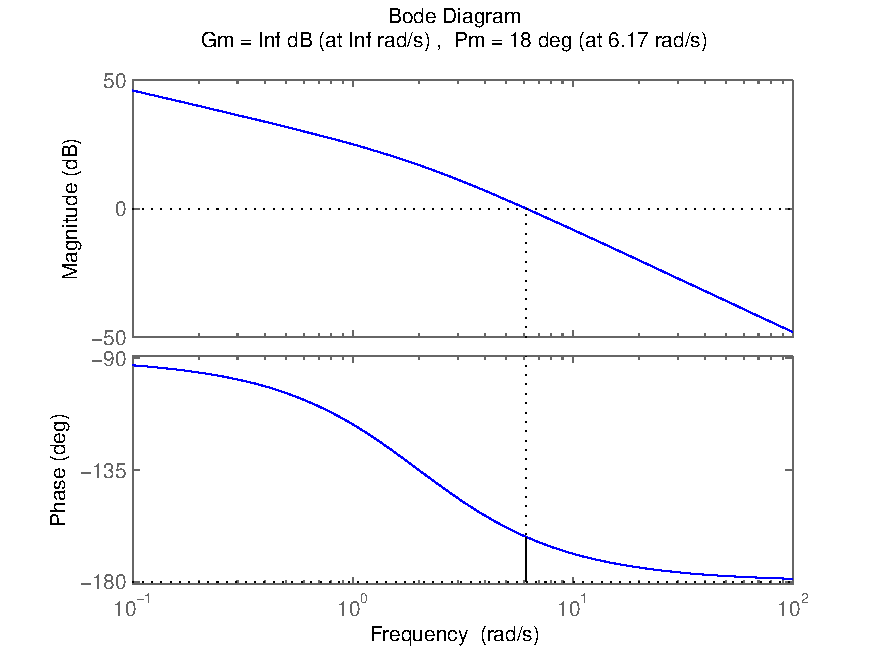
\includegraphics[width=0.7
		\linewidth]{leadstep1better}
	\end{figure}
\end{frame}

\begin{frame}
\begin{exampleblock}{Step 2: alternative way}
Calculation of phase margin without phase diagram: \\
We need the frequency where the magnitude is 0 dB. \\So, $20\log \mid K\alpha P(s) \mid = 0$
$\Rightarrow \mid K\alpha P(s) \mid = 1$
$\Rightarrow \mid P(s) \mid = 0.1$ \\
When substituting $s = j\omega$ and calculating the modulus of the complex number at the left side, the equation becomes: \\
\vspace{0.1 cm}
 $\left(\frac{-4\omega}{\omega \left( 4 + \omega^2\right)} \right) ^2 + \left( \frac{-8}{\omega \left( 4 + \omega^2 \right) }\right) ^2 = 0.01$. \\
\vspace{0.1 cm}
This equation has just one real positive solution: $\omega = 6.168$.\\
Now, we have the right frequency. We can calculate $10P(6.168j)$ = -0.951 - 0.308j. With the arctangent, we find that the phase of $10P(6.168j)$ is equal to $-162.05\,^{\circ}$. The phase margin is the difference between this value and $-180\,^{\circ}$, so the phase margin is equal to $17.95\,^{\circ}$.
\end{exampleblock}
\end{frame}

\begin{frame}
\begin{exampleblock}{Step 3}
	$\phi_m = \phi + 5\,^{\circ} = 37\,^{\circ}$
\end{exampleblock}
	\begin{exampleblock}{Step 4}
		$\alpha = \frac{1 - \sin \phi_m}{1 + \sin \phi_m} = 0.24$ \\
		From step 1, we know that $K = \frac{10}{\alpha} = 42$
	\end{exampleblock}
	\begin{exampleblock}{Step 5}
		Find $\omega_m$, the frequency at which the gain is $-20\log\left( K\sqrt{\alpha}\right) $ dB. 
		$GCF\left( P(s)K\sqrt{\alpha}\right) = \omega_m = 9 \frac{rad}{s}$ (see the Bode Diagram of  $P(s)K\sqrt{\alpha}$ in the next slide)
	\end{exampleblock}
\end{frame}

\begin{frame}
	\begin{figure}
		\centering
		\includegraphics[width=0.7
		\linewidth]{exampleleadsteptangent}
	\end{figure}
\end{frame}

\begin{frame}
	\begin{exampleblock}{Step 6}
		$\tau = \frac{1}{\omega_m\sqrt{\alpha}} = 0.23$
	\end{exampleblock}
	\begin{exampleblock}{Step 7}
	We verify whether or not our solution is correct. We plot the Bode Diagram of $ \frac{4}{s(s+2)} K \frac{s+\frac{1}{\tau}}{s+\frac{1}{\alpha\tau}}$ with the $\alpha$, $\tau$ and K we found. (see next slide) \\
	We see that: 
	\begin{itemize}
		\item the phase margin is indeed more than $50\,^{\circ}$ 
		\item the new gain crossover frequency is indeed about $9\frac{rad}{s}$
		\item the static velocity error constant is all right: $K_v = \lim_{s \to 0} sP(s)C(s) = 20$
	\end{itemize} 
	\end{exampleblock}
\end{frame}

\begin{frame}
\begin{figure}
	\centering
	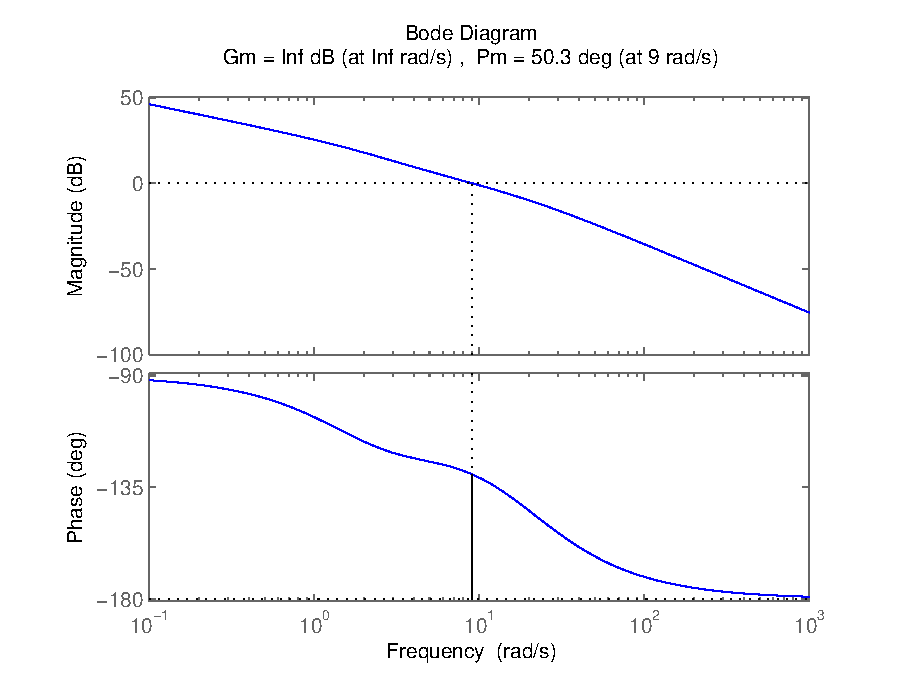
\includegraphics[width=0.7
	\linewidth]{leadstep7better}
\end{figure}
\end{frame}

\begin{frame}
	\begin{exampleblock}{Comparing compensated system vs non-compensated system}
	\begin{figure}
		\centering
		\includegraphics[width=0.7
		\linewidth]{leadcomparingbetter}
	\end{figure}
	\end{exampleblock}
\end{frame}

\section{Lag compensators}

\begin{frame}
	\frametitle{Lag compensators}
	\begin{block}{Transfer function}
		$C(s) = K\frac{s + \frac{1}{\tau}}{s + \frac{1}{\beta\tau}} = K\beta\frac{\tau s + 1}{\beta \tau s + 1}$ with $\beta  \textgreater  1$
	\end{block}
	\begin{block}{Bode Diagram}
		Example with $K$ = 1, $\beta$ = 10 and $\tau$ = 1 (see next slide) \\ 
		Magnitude of the lag compensator: 
		\begin{itemize}
			\item becomes 10 (= 20 dB) for small frequencies
			\item becomes unity (= 0 dB) for high frequencies
		\end{itemize}
		$\Rightarrow$ A lag compensator is a {\bf low-pass filter}.
		
	\end{block}
\end{frame}

\begin{frame}
\frametitle{Lag compensators}
\begin{block}{Bode Diagram}
	\begin{figure}
		\centering
		\includegraphics[width=0.5
		\linewidth]{bodelagislowpass}
	\end{figure}
\end{block}
\end{frame}

\begin{frame}
	\frametitle{Lag compensators}
	\begin{block}{Impact of lag compensators: Bode Diagram}
	\begin{itemize}
	\item The primary function of a lag compensator is to provide attenuation in the high-frequency
	range to give a system sufficient phase margin. The phase-lag characteristic
	is of no consequence in lag compensation.
	\item A lag compensator decreases the bandwidth/speed of response: 
	\begin{itemize}
		\item good to reduce the impact of high-frequency noise 
		\item bad if you want the system to react fast $\Rightarrow$ use lead compensator
	\end{itemize}
	\end{itemize}
	\end{block}
\end{frame}

		

\begin{frame}
	\frametitle{Lag compensators}
	\begin{block}{Design with Bode plots}
		\begin{itemize}
		\item Increase of phase margin implies decrease of the magnitude at high frequencies 
		\item Decrease of the steady state error implies increase of the DC-level ($\omega$ = 0)
		\end{itemize}
		A lag compensator can realize both conditions.
		\begin{itemize}
			\item At high frequencies, the gain becomes:
			$\lim_{s \to \infty} K\frac{s + \frac{1}{\tau}}{s + \frac{1}{\beta\tau}} = K$ 
			\item At $\omega$ = 0, the gain becomes: $\lim_{s \to 0} K\frac{s + \frac{1}{\tau}}{s + \frac{1}{\beta\tau}} = K\beta$
		\end{itemize}
	\end{block}
\end{frame}


\begin{frame}
\frametitle{Design with Bode plots}
\begin{block}{Step 1}
	\begin{itemize}
	\item Determine $K\beta$ in a similar way as we found $K\alpha$ for the lead compensator.
	\item Translate your steady state requirement in terms of the error constant:
	\begin{itemize}
		\item $K_p = \lim_{s \to 0} P(s)C(s)$
		\item $K_v = \lim_{s \to 0} sP(s)C(s)$
		\item $K_a = \lim_{s \to 0} s^2P(s)C(s)$
	\end{itemize}
	\item With this $K_p/K_v/K_a$, we determine $K\beta$.
	\item Check whether $K\beta P(s)$ satisfies the specifications on phase and gain margins.
	\end{itemize}
\end{block}
\end{frame}

\begin{frame}
\frametitle{Design with Bode plots}
\begin{block}{Step 2}
	\begin{itemize}
	\item Take the frequency ($\omega$) at which $P(s)$ has the desired phase ($-180\,^{\circ}$ + the desired phase margin + a safety factor of $10\,^{\circ}$). The addition of $10\,^{\circ}$ compensates for the phase lag of the lag compensator. Choose this frequency as the new gain crossover frequency $\omega_{GCF}$.
	\end{itemize}
\end{block}
\end{frame}

\begin{frame}
\frametitle{Design with Bode plots}
\begin{block}{Step 3}Choose the corner frequency $\omega = \frac{1}{\tau}$ one decade below $\omega_{GCF}$ to avoid bad effects of phase lag due to the lag compensator. Notice that we choose the compensator pole and zero sufficiently small. Thus the phase lag occurs at the low-frequency region so that it will not affect the phase margin.
\end{block}
\end{frame}

\begin{frame}
\frametitle{Design with Bode plots}
\begin{block}{Step 4}
	\begin{itemize}
\item Determine the attenuation $Q$ (in dB!) necessary to bring the magnitude curve down to 0 dB at $\omega_{GCF}$. 
\item Compute $\beta = 10^{(\frac{-Q}{20})}$.
\end{itemize}

\end{block}
\begin{block}{Step 5}
	\begin{itemize}
\item 	We just have calculated $\beta$ (step 4) and we know $K\beta$ (step 1), so it is possible to determine $K$.
\item 	Verify the behavior of the resulting system.
\end{itemize}
\end{block}
\end{frame}


\begin{frame}
\begin{example}
Given the system $P(s) = \frac{1}{s(s+1)(s+2)}$ with Bode Diagram below.
We want a static velocity error constant $K_v =\frac{5}{sec}$ and a PM $ \geq 40\,^{\circ}$.
\begin{figure}
	\centering
	\includegraphics[width=0.5
	\linewidth]{examplelag}
\end{figure}
\end{example}
\end{frame}

\begin{frame}
\begin{exampleblock}{Step 1}
	\begin{itemize}
	\item Steady state requirement: $K_v = \frac{5}{sec}$ \\
	$\Rightarrow \lim_{s \to 0} sP(s)C(s) = \frac{1}{2}\lim_{s \to 0} C(s) = \frac{5}{sec} \Rightarrow K\beta = 10$
	\item Would a proportional controller with gain $K\beta$ suffice? To answer this, we must have a look at the Bode plot of $K\beta P(s)$ (see next slide). \\
	$\Rightarrow$ Does not suffice! Adding a gain of $10 = 20 dB$ to get the right steady state error, the phase margin would become negative. In other words, at the frequency where the magnitude of $K\beta P(s)$ equals 0 dB, the phase is less than $-180\,^{\circ}$ which means the system would become unstable.
	\end{itemize}
\end{exampleblock}
\end{frame}

\begin{frame}
\begin{exampleblock}{Step 1}
\begin{figure}
	\centering
	\includegraphics[width=0.6
	\linewidth]{lagstep1better}
\end{figure}	
\end{exampleblock}
\end{frame}

\begin{frame}
\begin{exampleblock}{Step 2}
	\begin{itemize}

\item Determine the desired phase \\ $phase = -180\,^{\circ} + 40\,^{\circ} + 10\,^{\circ} = -130\,^{\circ}$ \\
\item $P(s)$ has the desired phase at a frequency of about $\omega_{GCF}$ = $0.5 \frac{rad}{s}$. (see Bode Diagram of $P(s)$) \\
	\end{itemize}
\end{exampleblock}
\begin{exampleblock}{Step 3}
	\begin{itemize}
		\item We take $\omega$ one decade below $\omega_{GCF}$, so $\omega = 0.05 \frac{rad}{s}$. 
		\item We compute $\tau = \frac{1}{\omega} = 20$.
	\end{itemize}
\end{exampleblock}
\end{frame}

\begin{frame}
\begin{exampleblock}{Step 4}
\begin{itemize}
\item To have an amplitude of $0 dB$ at $\omega_{GCF}$ in $K\beta P(s)$, we need an attenuation $Q = -20 dB$.
\item $\beta = 10^{\frac{-Q}{20}} = 10$
\end{itemize}
\end{exampleblock}
\begin{exampleblock}{Step 5}
\begin{itemize}
\item From the results of step 1 and step 4, we find $K = 1$.
\item We find $C(s) = \frac{s + 0.05}{s + 0.005}$. \\ We verify the behavior of $P(s)C(s) = \frac{1}{s(s+1)(s+2)}\frac{s + 0.05}{s + 0.005}$ on its Bode Diagram (see next slide). \\
The phase margin is indeed greater than $40\,^{\circ}$.
\end{itemize}
\end{exampleblock}
\end{frame}

\begin{frame}
\begin{exampleblock}{Step 5 continued}
\begin{figure}
	\centering
	\includegraphics[width=0.6
	\linewidth]{lagstep5better}
\end{figure}
\end{exampleblock}
\end{frame}

\begin{frame}
\begin{exampleblock}{Comparing compensated system vs non-compensated system}
\begin{figure}
	\centering
	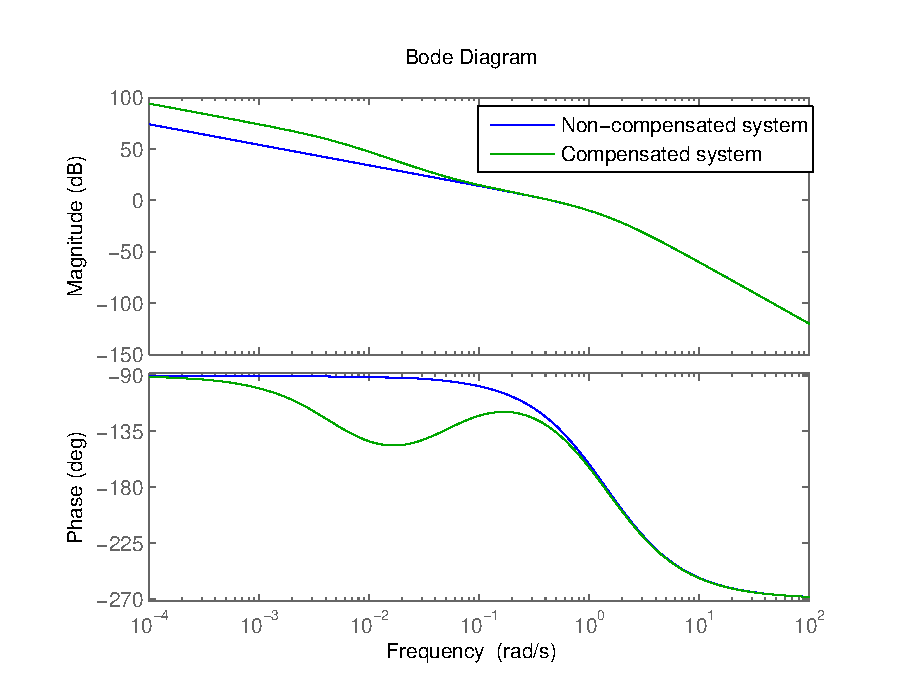
\includegraphics[width=0.6
	\linewidth]{lagcomparingbetter}
\end{figure}
\end{exampleblock}
\end{frame}



\section{Lag-lead compensators}

\begin{frame}
\frametitle{Lag-lead compensators}
\begin{block}{Introduction}
	In some cases you would want to combine the effects of a lag and a lead compensator:\\
		In most cases a lead compensator is more fit to increase the phase margin and a lag compensator is better at 	decreasing the steady state error.
\end{block}
\end{frame}

\begin{frame}
\frametitle{Lag-lead compensators}
\begin{block}{Transfer function}
	$C(s) = K\frac{s + \frac{1}{\tau_1}}{s + \frac{1}{\alpha\tau_1}}\frac{s + \frac{1}{\tau_2}}{s + \frac{1}{\beta\tau_2}}$ with $\beta \textgreater 1$, $0 \textless \alpha \textless 1$, $\tau_1 \textless \tau_2$ \\
	Usually, we take $\beta$ = $\frac{1}{\alpha}$, but that is not necessary. \\
	\begin{itemize}
	\item The term $\frac{s + \frac{1}{\tau_1}}{s + \frac{1}{\alpha\tau_1}}$ produces the effect of the lead network.
	\item The term $\frac{s + \frac{1}{\tau_2}}{s + \frac{1}{\beta\tau_2}}$ produces the effect of the lag network.
	\item Zeros: $\frac{1}{\tau_1}$ and $\frac{1}{\tau_2}$
	\item Poles: $\frac{1}{\alpha \tau_1}$ and $\frac{1}{\beta \tau_2}$
	\end{itemize}
\end{block}

\end{frame}

\begin{frame}
\frametitle{Lag-lead compensators}
\begin{block}{Bode Diagram}
Example with K = 10, $\alpha$ = 0.1, $\beta$ = 10, $\tau_1$ = 0.01, $\tau_2$ = 10 (see next slide) \\
Magnitude of lag-lead compensator:
\begin{itemize}
\item becomes 10 (= 20 dB) at low frequencies
\item becomes unity (= 0 dB) at frequencies of about $1 \frac{rad}{s}$ to $10 \frac{rad}{s}$
\item becomes 10 (= 20 dB) at high frequencies
\end{itemize}
$\Rightarrow$ A lag-lead compensator is a {\bf band stop filter}. \\
Explanation: $\beta \tau_2 \textgreater \tau_2 \textgreater \tau_1 \textgreater \alpha \tau_1$ \\
$\Rightarrow \frac{1}{\beta \tau_2} \textless \frac{1}{\tau_2} \textless \frac{1}{\tau_1} \textless \frac{1}{\alpha \tau_1}$ \\
$\Rightarrow$ $pole_1 \textless zero_1 \textless zero_2 \textless pole_2$
\end{block}
\end{frame}

\begin{frame}
\frametitle{Lag-lead compensators}
\begin{block}{Bode Diagram}
\begin{figure}
	\centering
	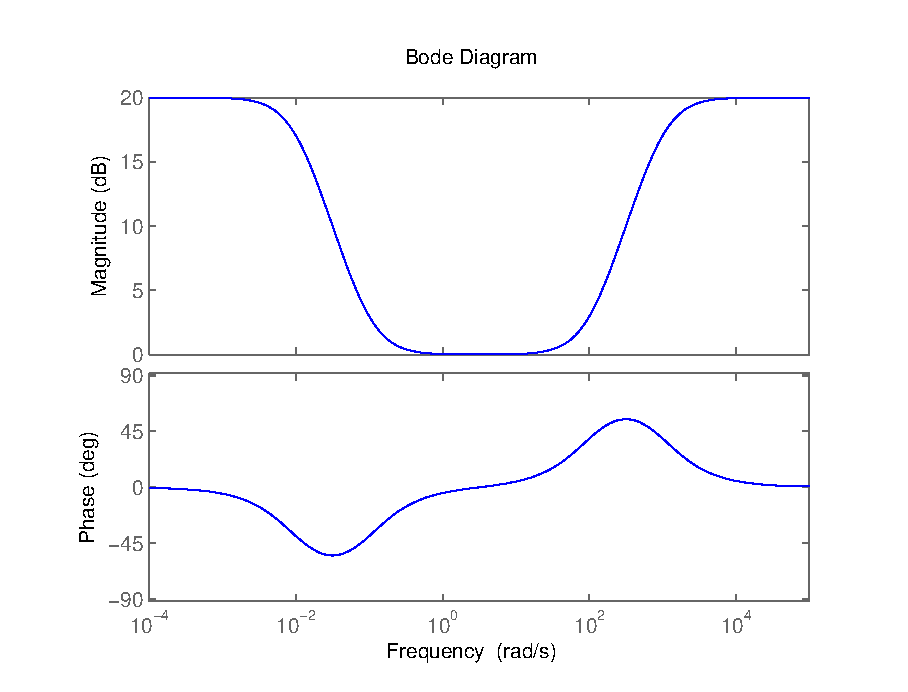
\includegraphics[width=0.5
	\linewidth]{laglead}
\end{figure}	
\end{block}
\end{frame}

\begin{frame}
\frametitle{Lag-lead compensators}	\begin{block}{Bode Diagram}
	Both the good properties of a lag and a lead compensator are used (see the Bode Diagram in the previous slide):
	\begin{itemize}
	\item At low frequencies, the lag compensator is meant to decrease the steady state error.
	\item At high frequencies, the lead compensator is meant to increase the phase margin.
	\end{itemize}
\end{block}
\end{frame}

\begin{frame}
\frametitle{Lag-lead compensators}
\begin{block}{Design with Bode plots}
	The
	design of a lag-lead compensator by the frequency-response approach is based on the
	combination of the design techniques discussed under lead compensation and lag
	compensation.
\end{block}
\begin{block}{Disadvantage}
	The disadvantage of a lag-lead compensator over a lag compensator or a lead compensator is its increased complexity, and hence cost (the same way a lag or lead compensator is more complex/costly than a proportional controller).
\end{block}
\end{frame}

\section{Comparison lead, lag and lag-lead compensators}

\begin{frame}
\frametitle{Comparison lead, lag and lag-lead compensators}
\begin{block}{Method}
\begin{itemize}
\item Lead compensation achieves the desired result through the merits of its phase lead
contribution.
\item Lag compensation accomplishes the result through the merits of its attenuation property at high frequencies.
\end{itemize}
\end{block}
\end{frame}

\begin{frame}
\frametitle{Comparison lead, lag and lag-lead compensators}
\begin{block}{Bandwidth}
Lead compensators are commonly used for improving stability margins and yields a higher gain crossover frequency than it is possible with lag compensation. The higher gain crossover frequency means a larger bandwidth.
\begin{itemize}
\item Advantage: reduction in the settling time $\Rightarrow$ fast response
\item Disadvantage: it makes the system more susceptible to noise because of
an increase in the high-frequency gain. 
\end{itemize}
\end{block}
\end{frame}

\begin{frame}
\frametitle{Comparison lead, lag and lag-lead compensators}
\begin{block}{Gain}
Lead compensation requires an additional increase in gain to offset the attenuation
inherent in the lead network. \\
$\Rightarrow$ Lead compensation will require
a larger gain than that required by lag compensation.
\end{block}
\begin{block}{Large control actions}
The lead compensation may generate large control actions in the system, which might lead to saturation in the system.
\end{block}
\end{frame}

\begin{frame}
	\frametitle{Comparison lead, lag and lag-lead compensators}
\begin{block}{High and low frequencies}
Lag compensation reduces the system gain at higher frequencies without reducing
the system gain at lower frequencies. Since the system bandwidth is reduced, the system has a slower speed to response. 
Thanks to this, the total system gain can be increased, as well as the low-frequency gain and the steady state accuracy can be improved. Also, any high-frequency
noise involved in the system is attenuated.
\end{block}
\begin{block}{Transient response}
Lag compensation will introduce a pole-zero combination near the origin that will
generate a long tail with small amplitude in the transient response.
\end{block}
\end{frame}

\begin{frame}
\frametitle{Comparison lead, lag and lag-lead compensators}
\begin{block}{Lag-lead compensators}
If both fast responses and good static accuracy are desired, a lag-lead compensator
may be employed. By use of the lag-lead compensator, the low-frequency gain can
be increased (which means an improvement in steady state accuracy), while at the
same time the system bandwidth and stability margins can be increased.
\end{block}
\end{frame}





